% Options for packages loaded elsewhere
% Options for packages loaded elsewhere
\PassOptionsToPackage{unicode}{hyperref}
\PassOptionsToPackage{hyphens}{url}
\PassOptionsToPackage{dvipsnames,svgnames,x11names}{xcolor}
%
\documentclass[
  letterpaper,
  DIV=11,
  numbers=noendperiod,
  oneside]{scrartcl}
\usepackage{xcolor}
\usepackage[left=1in,marginparwidth=2.0666666666667in,textwidth=4.1333333333333in,marginparsep=0.3in]{geometry}
\usepackage{amsmath,amssymb}
\setcounter{secnumdepth}{-\maxdimen} % remove section numbering
\usepackage{iftex}
\ifPDFTeX
  \usepackage[T1]{fontenc}
  \usepackage[utf8]{inputenc}
  \usepackage{textcomp} % provide euro and other symbols
\else % if luatex or xetex
  \usepackage{unicode-math} % this also loads fontspec
  \defaultfontfeatures{Scale=MatchLowercase}
  \defaultfontfeatures[\rmfamily]{Ligatures=TeX,Scale=1}
\fi
\usepackage{lmodern}
\ifPDFTeX\else
  % xetex/luatex font selection
\fi
% Use upquote if available, for straight quotes in verbatim environments
\IfFileExists{upquote.sty}{\usepackage{upquote}}{}
\IfFileExists{microtype.sty}{% use microtype if available
  \usepackage[]{microtype}
  \UseMicrotypeSet[protrusion]{basicmath} % disable protrusion for tt fonts
}{}
\makeatletter
\@ifundefined{KOMAClassName}{% if non-KOMA class
  \IfFileExists{parskip.sty}{%
    \usepackage{parskip}
  }{% else
    \setlength{\parindent}{0pt}
    \setlength{\parskip}{6pt plus 2pt minus 1pt}}
}{% if KOMA class
  \KOMAoptions{parskip=half}}
\makeatother
% Make \paragraph and \subparagraph free-standing
\makeatletter
\ifx\paragraph\undefined\else
  \let\oldparagraph\paragraph
  \renewcommand{\paragraph}{
    \@ifstar
      \xxxParagraphStar
      \xxxParagraphNoStar
  }
  \newcommand{\xxxParagraphStar}[1]{\oldparagraph*{#1}\mbox{}}
  \newcommand{\xxxParagraphNoStar}[1]{\oldparagraph{#1}\mbox{}}
\fi
\ifx\subparagraph\undefined\else
  \let\oldsubparagraph\subparagraph
  \renewcommand{\subparagraph}{
    \@ifstar
      \xxxSubParagraphStar
      \xxxSubParagraphNoStar
  }
  \newcommand{\xxxSubParagraphStar}[1]{\oldsubparagraph*{#1}\mbox{}}
  \newcommand{\xxxSubParagraphNoStar}[1]{\oldsubparagraph{#1}\mbox{}}
\fi
\makeatother


\usepackage{longtable,booktabs,array}
\newcounter{none} % for unnumbered tables
\usepackage{calc} % for calculating minipage widths
% Correct order of tables after \paragraph or \subparagraph
\usepackage{etoolbox}
\makeatletter
\patchcmd\longtable{\par}{\if@noskipsec\mbox{}\fi\par}{}{}
\makeatother
% Allow footnotes in longtable head/foot
\IfFileExists{footnotehyper.sty}{\usepackage{footnotehyper}}{\usepackage{footnote}}
\makesavenoteenv{longtable}
\usepackage{graphicx}
\makeatletter
\newsavebox\pandoc@box
\newcommand*\pandocbounded[1]{% scales image to fit in text height/width
  \sbox\pandoc@box{#1}%
  \Gscale@div\@tempa{\textheight}{\dimexpr\ht\pandoc@box+\dp\pandoc@box\relax}%
  \Gscale@div\@tempb{\linewidth}{\wd\pandoc@box}%
  \ifdim\@tempb\p@<\@tempa\p@\let\@tempa\@tempb\fi% select the smaller of both
  \ifdim\@tempa\p@<\p@\scalebox{\@tempa}{\usebox\pandoc@box}%
  \else\usebox{\pandoc@box}%
  \fi%
}
% Set default figure placement to htbp
\def\fps@figure{htbp}
\makeatother


% definitions for citeproc citations
\NewDocumentCommand\citeproctext{}{}
\NewDocumentCommand\citeproc{mm}{%
  \begingroup\def\citeproctext{#2}\cite{#1}\endgroup}
\makeatletter
 % allow citations to break across lines
 \let\@cite@ofmt\@firstofone
 % avoid brackets around text for \cite:
 \def\@biblabel#1{}
 \def\@cite#1#2{{#1\if@tempswa , #2\fi}}
\makeatother
\newlength{\cslhangindent}
\setlength{\cslhangindent}{1.5em}
\newlength{\csllabelwidth}
\setlength{\csllabelwidth}{3em}
\newenvironment{CSLReferences}[2] % #1 hanging-indent, #2 entry-spacing
 {\begin{list}{}{%
  \setlength{\itemindent}{0pt}
  \setlength{\leftmargin}{0pt}
  \setlength{\parsep}{0pt}
  % turn on hanging indent if param 1 is 1
  \ifodd #1
   \setlength{\leftmargin}{\cslhangindent}
   \setlength{\itemindent}{-1\cslhangindent}
  \fi
  % set entry spacing
  \setlength{\itemsep}{#2\baselineskip}}}
 {\end{list}}
\usepackage{calc}
\newcommand{\CSLBlock}[1]{\hfill\break\parbox[t]{\linewidth}{\strut\ignorespaces#1\strut}}
\newcommand{\CSLLeftMargin}[1]{\parbox[t]{\csllabelwidth}{\strut#1\strut}}
\newcommand{\CSLRightInline}[1]{\parbox[t]{\linewidth - \csllabelwidth}{\strut#1\strut}}
\newcommand{\CSLIndent}[1]{\hspace{\cslhangindent}#1}



\setlength{\emergencystretch}{3em} % prevent overfull lines

\providecommand{\tightlist}{%
  \setlength{\itemsep}{0pt}\setlength{\parskip}{0pt}}



 


\KOMAoption{captions}{tableheading}
\makeatletter
\@ifpackageloaded{caption}{}{\usepackage{caption}}
\AtBeginDocument{%
\ifdefined\contentsname
  \renewcommand*\contentsname{Table of contents}
\else
  \newcommand\contentsname{Table of contents}
\fi
\ifdefined\listfigurename
  \renewcommand*\listfigurename{List of Figures}
\else
  \newcommand\listfigurename{List of Figures}
\fi
\ifdefined\listtablename
  \renewcommand*\listtablename{List of Tables}
\else
  \newcommand\listtablename{List of Tables}
\fi
\ifdefined\figurename
  \renewcommand*\figurename{Figure}
\else
  \newcommand\figurename{Figure}
\fi
\ifdefined\tablename
  \renewcommand*\tablename{Table}
\else
  \newcommand\tablename{Table}
\fi
}
\@ifpackageloaded{float}{}{\usepackage{float}}
\floatstyle{ruled}
\@ifundefined{c@chapter}{\newfloat{codelisting}{h}{lop}}{\newfloat{codelisting}{h}{lop}[chapter]}
\floatname{codelisting}{Listing}
\newcommand*\listoflistings{\listof{codelisting}{List of Listings}}
\makeatother
\makeatletter
\makeatother
\makeatletter
\@ifpackageloaded{caption}{}{\usepackage{caption}}
\@ifpackageloaded{subcaption}{}{\usepackage{subcaption}}
\makeatother
\makeatletter
\@ifpackageloaded{sidenotes}{}{\usepackage{sidenotes}}
\@ifpackageloaded{marginnote}{}{\usepackage{marginnote}}
\makeatother
\usepackage{bookmark}
\IfFileExists{xurl.sty}{\usepackage{xurl}}{} % add URL line breaks if available
\urlstyle{same}
% fallback for those not using the hyperref driver hyperxmp:
\makeatletter
\@ifundefined{xmpquote}{\newcommand{\xmpquote}[1]{#1}}{}
\makeatother
\hypersetup{
  pdftitle={SOC 105 Lecture Notes},
  colorlinks=true,
  linkcolor={blue},
  filecolor={Maroon},
  citecolor={Blue},
  urlcolor={Blue},
  pdfcreator={LaTeX via pandoc}}


\title{SOC 105 Lecture Notes}
\author{}
\date{}
\begin{document}
\maketitle


\begin{figure}[H]

{\centering 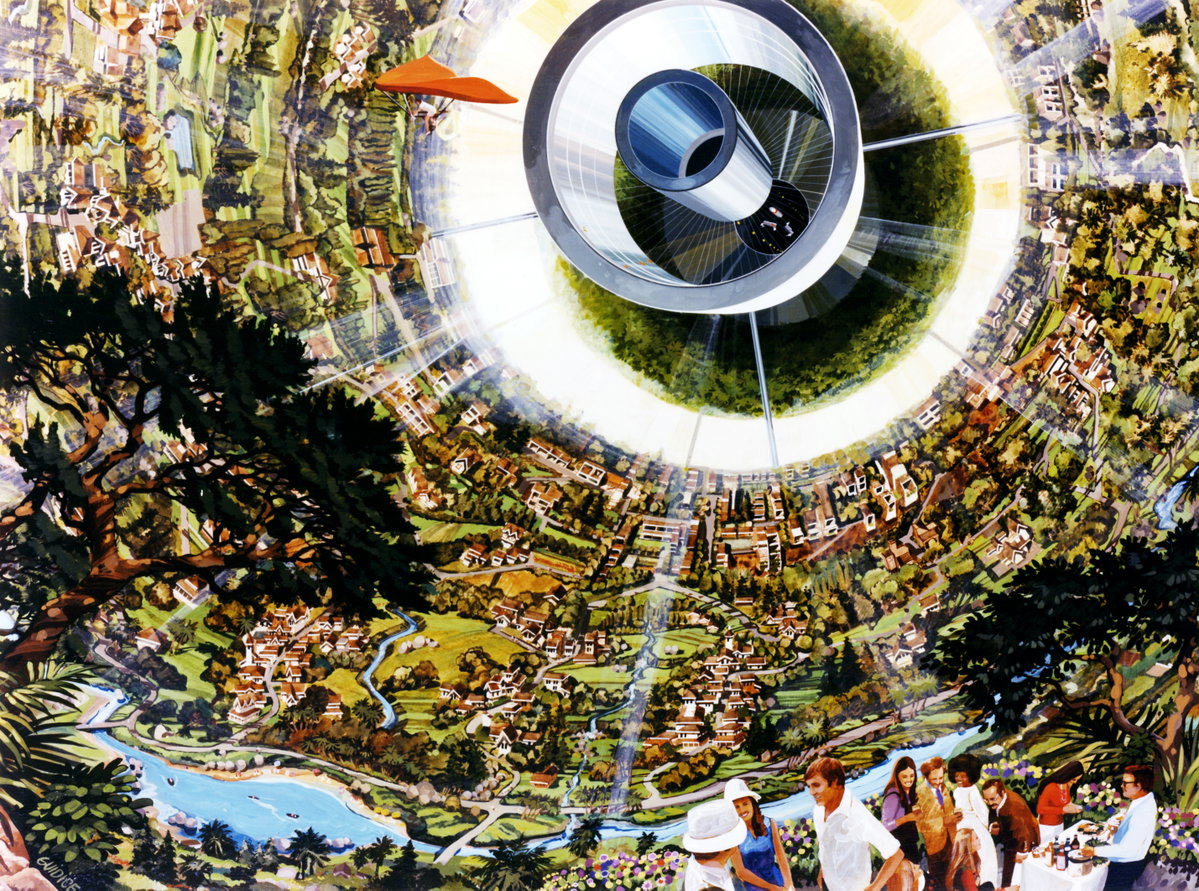
\includegraphics[width=6.59375in,height=\textheight,keepaspectratio]{images/0_header_3.jpg}

}

\caption{``Bernal Interior'' by Rick Guidice, ca. 1970s.
\href{https://pdimagearchive.org/images/33f8f1c3-0565-4157-9ef8-9dd887eb881e/}{Source}}

\end{figure}%

\section{Welcome!}\label{welcome}

Welcome to the lecture notes for SOC 105 at Stony Brook University! My
name is Nick Wilson, and I've been teaching this course here since the
Fall of 2016. Until now, I employed a regular textbook, but this
semester have decided to transition to these typed lecture notes.

\marginnote{\begin{footnotesize}

Formally, I am an Associate Professor of Sociology at Stony Brook
University, but I don't particularly like such trappings, especially in
person, so please just call me ``Nick.'' Note, however, that many of
your professors want to be addressed formally!

\end{footnotesize}}

\subsection{Why These Notes?}\label{why-these-notes}

Over the course of teaching introduction to sociology (with enrollments
of around 250 students), I've grown increasingly dissatisfied with the
textbook I was using, and, indeed, any one that I could find. This was
for several reasons.

\begin{enumerate}
\def\labelenumi{\arabic{enumi}.}
\tightlist
\item
  \textbf{Cost.} Most textbooks seem unjustifiably expensive today. A
  quick glance at Amazon shows that they can range from \$30 to over
  \$150 to buy, and still a substantial amount of money to rent.
\item
  \textbf{Quality.} While most textbooks are nominally written by
  well-known academics, as we will see, sociology is a notoriously
  difficult subject to even introduce, so the quality of textbooks
  varies wildly, both within and among the different offerings.
\item
  \textbf{Voice.} You will find that I prefer to write prose in a
  direct, conversational, active style, and this is something that is
  surprisingly hard to find in a textbook. Even ones that are written
  ``simply'' tend to overdo the passive voice, pointlessly elevate
  jargon, exaggerate the unity and certainty of sociology's findings,
  and employ other false trappings of scientific authority.\sidenote{\footnotesize I
    think I am most influenced by the writing styles of George Orwell
    (2013), Christopher Lasch (2002), and Strunk and White's (2009).}
\item
  \textbf{Datedness.} Because traditional textbooks take so long to
  conceive, write, vet, and physically produce, they are usually
  surprisingly dated by the time they are published.\sidenote{\footnotesize For
    instance, it is only now that textbooks are even acknowledging, much
    less considering the impact of, COVID-19.}
\item
  \textbf{Intellectual divergence.} Finally, I also noticed that I
  increasingly disagreed with most available textbooks. I especially
  chafed at them oversimplifying sociology. In my view, the field is
  ambiguous, difficult, and challenging; indeed, it is one of the
  hardest sciences to practice, because it has the most complex object
  of study---society itself. By extension, I have come to believe that
  an introduction to sociology should be clear, but not simple.
\end{enumerate}

With those reasons in mind, beginning in the summer of 2024 I decided to
transform and extend my lecture slides into these notes, and I worked
intensively to complete the first draft of these notes in the summer of
2026.

\section{Organization of These Notes}\label{organization-of-these-notes}

After this Introduction, the notes are divided into four main parts.

\subsection{Part I: Orientation}\label{part-i-orientation}

In Part I, I discuss sociology's distinctive intellectual style and
heritage,\sidenote{\footnotesize Chapter 1:
  \href{./chapters/Ch_1_Imagination.qmd}{Imagination}.} its place among
other disciplines,\sidenote{\footnotesize Chapter 2:
  \href{./chapters/Ch_2_Discipline.qmd}{Discipline}.} and then its
(several) methods and their benefits and challenges of each.\sidenote{\footnotesize Chapter
  3: \href{./chapters/Ch_3_Method.qmd}{Methods}.}

\subsection{Part II: Conceptual
Foundation}\label{part-ii-conceptual-foundation}

After that, since this a course meant to introduce you to the field, the
bulk of the notes, comprising six chapters, is in Part II, which oulines
what I consider to be the fundamental conceptual building blocks in
sociology. I think sociology is fundamentally oriented around the
intersection of meaning and action,\sidenote{\footnotesize Chapter 4:
  \href{./chapters/Ch_4_Meaning.qmd}{Meaning and Action}.} especially in
contexts of interaction,\sidenote{\footnotesize Chapter 5:
  \href{./chapters/Ch_5_Interaction.qmd}{Interaction}.} is usually
organized following social structures,\sidenote{\footnotesize Chapter 6:
  \href{./chapters/Ch_6_Structures.qmd}{Social Structure}.} the result
of which are qualities we have usually called identities or
selves.\sidenote{\footnotesize Chapter 7:
  \href{./chapters/Ch_7_Identity.qmd}{Identity}.} Finally, there are two
special characteristics of social structures that are such common
features of sociological analysis that they have become foundational:
that your place in social structures is not what it is only because of
everyone's agreement, but also because of power and
discipline;\sidenote{\footnotesize Chapter 8:
  \href{./chapters/Ch_8_Discipline.qmd}{Power and Discipline}.} and
that, especially in complex societies, almost every social structure
exhibits some form of inequality.\sidenote{\footnotesize Chapter 9:
  \href{./chapters/Ch_9_Inequality.qmd}{Inequality}.}

\subsection{Part III: Elaborations}\label{part-iii-elaborations}

Part III combines these building blocks, along with the two
world-historical shifts of central interest to sociologists (the
emergence and eventual dominance of capitalism and the rise,
transformation, and dissolution of large empires) to understand key
features of the era in which we live, ``modernity.'' The forces at work
in this era are different from what came before in critical ways, and
affect everything from our identities--our sense of race and
ethnicity,\sidenote{\footnotesize Chapter 10: \href{./chapters/Ch_10_Race.qmd}{Race
  and Ethnicity}.} gender and sexuality,\sidenote{\footnotesize Chapter 11:
  \href{./chapters/Ch_11_Gender.qmd}{Gender and Sexuality}.} and even
how we imagine our place in the world\sidenote{\footnotesize Chapter 12:
  \href{./chapters/Ch_12_Globalization.qmd}{Globalization}.}--and has
decisively reorganized our lives through political,\sidenote{\footnotesize Chapter 13:
  \href{./chapters/Ch_13_Politics.qmd}{Politics}.} economic,\sidenote{\footnotesize Chapter
  14: \href{./chapters/Ch_14_Economics.qmd}{Economics}.}
environmental,\sidenote{\footnotesize Chapter 15:
  \href{./chapters/Ch_15_Environment.qmd}{Environment}.} and even
biological\sidenote{\footnotesize Chapter 16:
  \href{./chapters/Ch_16_Health.qmd}{Health}.} change.

\section{How To Read These Notes (And Do Well In This
Course!)}\label{how-to-read-these-notes-and-do-well-in-this-course}

This way of communicating course content in SOC 105 is new to me, and
experimental, so I'm eager to hear your feedback as the semester
progresses. With that said, I've written these notes with a few ideas in
mind about how they integrate with other course materials (particularly
the exams and lectures), so I have some advice about how to make the
most out of these notes.

\subsection{Logical Flow}\label{logical-flow}

I've tried to keep each unit within these notes fairly tightly
self-contained, which means you \emph{should} be able to read each one
without having to read all of the others. At the same time, I've also
(especially at the beginning and end of each unit) tried to tie the
units together into a logical sequence, so you will also (hopefully)
understand a larger picture of \emph{why} particular units come before
and after one another, and why others are clustered together.

This duality implies that there are two levels on which you can
understand any given unit: first, on its own terms\sidenote{\footnotesize For
  instance, what do you learn about Race or Gender just by reading those
  units?}; and second, in the context of the mosaic of sociology as
represented by all the units together. Consequently, it is a good idea
to ask yourself two kinds of question when reading a unit:

\begin{quote}
What are the three or four main conceptual and empirical points I need
to know about the topic covered in the unit? How do empirical and
conceptual details in the unit relate back too these ``big'' points?
\end{quote}

and

\begin{quote}
How does this unit fit into the course? How does it help me understand
units that came before, and flow into those that follow it? How would my
understanding of other units change if I didn't know the information in
this one?
\end{quote}

\subsection{Marginal Helpers}\label{marginal-helpers}

Depending on how you are reading this overview, you will see a
more-or-less evident right hand column running alongside the main text.
In it, post three main things:

\marginnote{\begin{footnotesize}

\textbf{Boldface type} is a more noticeable form of text used to
emphasize important ideas or words.

\end{footnotesize}}

\begin{enumerate}
\def\labelenumi{\arabic{enumi}.}
\tightlist
\item
  \textbf{Asides}, both empirical or personal. (You'll just have to read
  them to find out which they are!) I don't consider these essential to
  grasping the main points of a chapter, but (I hope) they can add
  context for interested readers.
\item
  \textbf{Definitions.} Throughout the text, when you encounter a
  \textbf{boldface} term in the main column, I have tried to state a
  plain definition nearby\sidenote{\footnotesize Where \emph{exactly} the definitions
    are placed is partly a function of the underlying software used to
    render this text, and partly how you are viewing it.} in the
  right-hand column. This is both for your convenience (to alert you to
  key terms), but also so you can see the term both in its content (used
  in the main column) and abstracted out of that context to its most
  general form (in the right-hand column).\sidenote{\footnotesize You'll notice that
    an important exception to this rule is when I use boldface type to
    announce the key element of a list, like this one---I haven't given
    you definitions for ``asides'' or, well, ``definitions.''}
\item
  \textbf{Links and references.} Typically, the first time I discuss a
  data source, book or article in the text, you will see a reference to
  it in the right-hand column. Likewise, since sociology's empirical
  depth is virtually bottomless, I will sometimes also provide links and
  materials for further exploration by those who are interested.
\end{enumerate}

\subsection{How I test}\label{how-i-test}

I think that SOC 105---and particularly the way I organize and teach
it---is unusual among introductory college courses. There is \emph{very}
little memorization necessary to do well. Instead, I ask that you try to
\emph{grasp} key concepts and understand how they relate to the world
around us. Accordingly, I ask three classes of question on my exams
(which, by the way, are all multiple choice and taken in class on a
scantron sheet).

\begin{enumerate}
\def\labelenumi{\arabic{enumi}.}
\tightlist
\item
  \textbf{Conceptual questions.} I want to know whether you can
  reasonably tell the content of a concept in the course\sidenote{\footnotesize Like
    ``race,'' ``inequality,'' ``social order,'' ``bureaucracy'' and so
    on.} and tell whether it is different from other terms.\sidenote{\footnotesize I'd
    like to know whether you can differentiate among a ``formal'' and
    ``informal'' organization, for instance.} So my exams generally
  contain a good number of questions that ask you to both identify a
  concept given a description (and vice versa) as well as to tell the
  difference among key concepts.
\item
  \textbf{Application questions.} I also want to assess your ability to
  make connections between concepts and empirical material--you should
  be able to tell if an application of a concept is appropriate to some
  phenomenon, and what leverage it gives us in understanding
  it.\sidenote{\footnotesize For instance, ``capitalism'' would be a strange concept
    to use to think about an economic organization with no money or
    investment for profit, and some interactions are best seen through
    the lens of ``gender,'' while others might be less so.} Since I want
  to know how well you do this \emph{beyond} simply memorizing what I've
  talked about in the course, questions I ask on exams in this category
  will only rarely be from applications and examples I discussed in
  lecture or these notes. Usually, they will be something new.
\item
  \textbf{``Big'' empirical questions.} I \emph{hate} questions that
  require memorizing empirical details---this is no longer how any of us
  learn, process, or store information. When it comes to knowing and
  remembering facts about the world, I care far more that you're able to
  understand \emph{why that fact is significant} relevant to a
  particular purpose, concept, theory, or phemonenon. Thus I \emph{will}
  ask you factual questions that are highly relevant to concepts and
  phenomena in the different units, but I \emph{will not} ask about
  nit-picky, subtle differences.\sidenote{\footnotesize For instance, relative to
    education, I might ask whether ``very few,'' ``about half,'' or
    ``almost all'' of the U.S. population has a Ph.D.~degree. Knowing
    the answer makes a big difference in your understanding of the
    stakes of education in the U.S., but knowing whether the answer is
    1.4\% or 1.5\% of the population does not.}
\end{enumerate}

Two further comments are warranted. The first is that I \emph{really}
want you to be successful in this course.\sidenote{\footnotesize This is both because
  I think sociology is awesome and want to arouse your curiosity in it,
  and also because I have no reason to try and ``weed out'' anyone.}
Therefore, I will \emph{never} ask you a ``gotcha'' or trick question on
an exam. Almost always, the right answer is the obvious\sidenote{\footnotesize I am
  \emph{not} saying ``common-sense!'' There are important times where a
  sociological understanding of a word that we use in everyday life
  diverges quite a bit. So if you don't study and try to just wing an
  exam, you'll be disappointed.} one---provided you have studied!---so
you shouldn't agonize over the possibility that I'm playing mind games
with you.

Second, you may have already noted that conceptual questions,
application questions, and big empirical questions, even when they're
narrowed-down in the way I describe above, cover a huge amount of
logical ground. So how do you know \emph{which} concepts, applications,
and phenomena to focus on when you study? For a clue, notice that there
are basically three sources of information available to you in this
course: what you read before class, what I present on the slides in
class, and what I say about those slides and the reading. As you can see
from the below \hyperref[fig_exam]{diagram}, where these three sources
of information overlap is where \emph{I} would concentrate my focus!

\begin{figure}

{\centering \pandocbounded{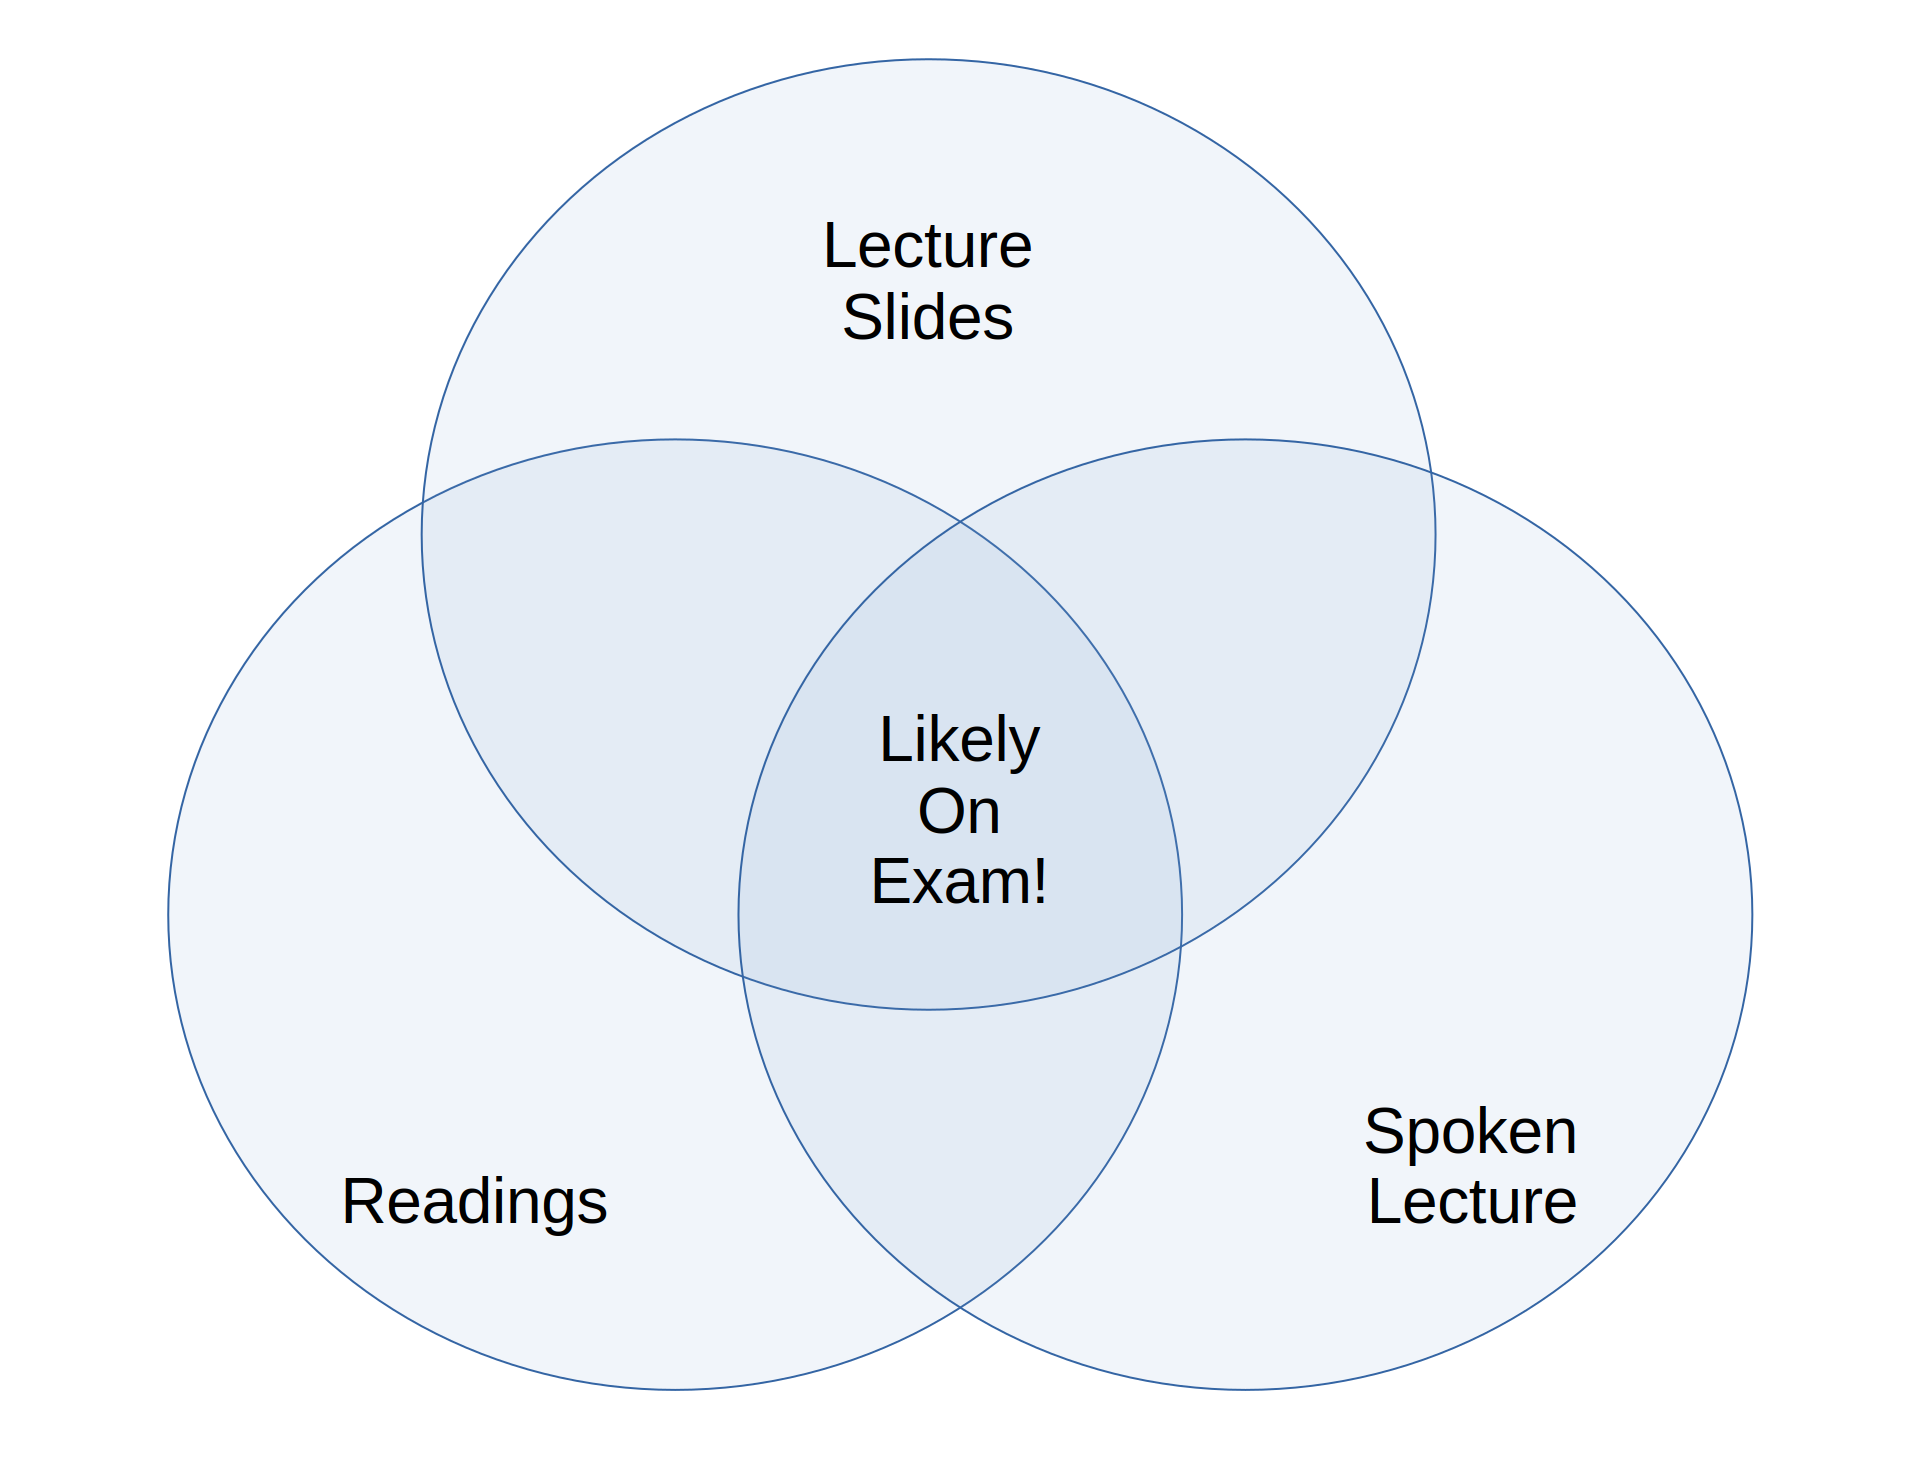
\includegraphics[keepaspectratio]{images/0_exam_diagram_2.png}}

}

\caption{Overlaps in sources of course information.}

\end{figure}%

\subsubsection{References}\label{references}

\protect\phantomsection\label{refs}
\begin{CSLReferences}{1}{1}
\bibitem[\citeproctext]{ref-laschPlainStyleGuide2002}
Lasch, Christopher. 2002.
\emph{\href{http://catdir.loc.gov/catdir/toc/fy035/2002019163.html}{Plain
Style: A Guide to Written {English}}}. edited by S. A. Weaver.
Philadelphia: University of Pennsylvania Press.

\bibitem[\citeproctext]{ref-orwellPoliticsEnglishLanguage2013}
Orwell, George. 2013. \emph{Politics and the {English Language}}. New
York: Penguin Classics.

\bibitem[\citeproctext]{ref-strunkjrElementsStyleFourth2009}
Strunk Jr, William, and E. B. White. 2009. \emph{The {Elements} of
{Style}, {Fourth Edition}}. New York, Munich: Pearson.

\end{CSLReferences}




\end{document}
